% PHY 317 Syllabus, Smith College, Fall 2026 -- Michael Lerner
%
% Tufte-handout, same preamble and section rhythm as the PHY 210 F2026
% syllabus (MathematicalPhysics/SyllabusAndFirstDay/2026/PHY210Syllabus.tex),
% so the two courses read as one instructor's. Content sources: the F2026
% calendar generator (make_fall2026_calendar.py -- the source of truth for
% every date), Will Raven's F2025 PHY 317 syllabus (exam design,
% redemption final, HW rubric with reflections, AI statement, the
% just-in-time prerequisites framing; all adapted and credited), and the
% PHY 210 policy text (PCCIs, late passes, recording, integrity).
%
% Red [TODO: ...] markers flag facts to fill in before distribution.
% Build: pdflatex PHY317Syllabus.tex  (twice, for margin-note placement)
\documentclass{tufte-handout}

\usepackage{amsmath}
\usepackage{amssymb}
\usepackage{graphicx}
\setkeys{Gin}{width=\linewidth,totalheight=\textheight,keepaspectratio}
\usepackage{booktabs}
\usepackage{units}
\usepackage{multicol}

% Underline every link (hyperref is loaded by tufte-handout).
\usepackage[normalem]{ulem}
\setlength{\emergencystretch}{1.5em}
\AtBeginDocument{%
  \let\syllabushref\href
  \renewcommand{\href}[2]{\syllabushref{#1}{\uline{#2}}}%
  \let\syllabusurl\url
  \renewcommand{\url}[1]{\uline{\syllabusurl{#1}}}%
}

\newcommand{\todonote}[1]{{\color{red} \textbf{[TODO: #1]}}}

\title{PHY 317: Classical Mechanics}
\author[Michael G. Lerner]{Michael G. Lerner}
\date{Smith College, Fall 2026}

\begin{document}

\maketitle

\marginnote[2\baselineskip]{%
  \textbf{Instructor:} Michael Lerner\\
  McConnell 303\\
  \href{mailto:mglerner@smith.edu}{mglerner@smith.edu}\\[4pt]
  \textbf{Class:} Sabin-Reed 308\\
  Mon 1:40--2:55, Wed \& Fri 1:20--2:35\\
  First meeting Wed Sep 9\\
  Last meeting Mon Dec 14\\[4pt]
  \textbf{Help Sessions (Office hours):} {\color{red}\textbf{TO BE SET}
  after the week-1 scheduling poll}. I also have an open-door policy:
  stop in whenever my door is open. That's most of the time.\\[4pt]
  \textbf{Text:} Taylor, \textit{Classical Mechanics} (University
  Science Books, 2005)\\[4pt]
  \textbf{Website:} Moodle\\
  \textbf{Python:} \url{https://posit.smith.edu} -- nothing to
  install or buy
}

\newthought{One of the great strengths} of classical mechanics is that
it is the subject where physics first learned to be systematic: the same
handful of ideas (Newton's laws, the conservation laws, and then the
principle of least action) describe a raindrop, a satellite, a spinning
top, and a chaotic pendulum. Newton's laws themselves are two courses
behind you. The primary objective of this course is to take them much
further than PHY 117 could -- forces that depend on velocity, systems of
many bodies, motion seen from accelerating and rotating frames -- and
then to rebuild the subject around the Lagrangian formulation, which is
the language that every theory you meet after this one is written in. A
significant secondary objective is to develop the fluency and the
checking habits (units, limiting cases, symmetry, a numerical solution
when the algebra gives out) that let you attack a mechanics problem you
have never seen before with confidence.
Concretely, by the end of this course you will be able to:
\begin{enumerate}
  \item Set up and solve the equations of motion for a mechanical
        system in whatever coordinates the problem wants -- Cartesian,
        polar, or your own generalized coordinates -- starting from
        Newton's laws or from a Lagrangian.
  \item Use the conservation laws (momentum, angular momentum, energy)
        as \emph{tools}, and know when each one applies and why.
  \item Analyze oscillations: damped, driven, resonant, coupled, and
        their normal modes.
  \item Solve the central-force problem and read an orbit off an
        effective potential; work in accelerating and rotating frames.
  \item Explain what chaos is and is not, and recognize it in a
        simulation.
  \item Use Python to solve equations of motion numerically, to check
        analytic results, and to explore what happens when the algebra
        gives out.
  \item Check your work the way physicists do: units, limiting cases,
        symmetry, and plugging the answer back in.
\end{enumerate}

\begin{marginfigure}
  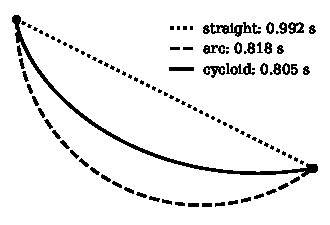
\includegraphics{brachistochrone}
  \caption{A bead slides without friction from the upper dot to the
    lower one. Which track gets it there fastest? Not the straight
    line. By week 8 you will be able to derive the winner (a cycloid)
    in about a page.}
  \label{fig:brach}
\end{marginfigure}

\section{Prerequisites}\label{sec:prereqs}

PHY 210 (Mathematical Methods) and PHY 215, or permission of the
instructor. This course builds directly on PHY 117 and a little of
PHY 118, and it uses the mathematics from PHY 210 constantly.

\newthought{Just-in-time review.} The course calendar on Moodle has a
``Prerequisites'' column that lists, for each new topic, the earlier
material it leans on (by Knight chapter for intro physics and by
Felder \& Felder chapter for math methods). There are two good ways to
use it: \emph{just-in-time} -- review those concepts before we get to
the topic -- or \emph{just-after-time} -- if a new idea is rough going,
use the list to find and shore up the foundation right after
class.\sidenote{This framing, and the column itself, are Will Raven's,
from his Fall 2025 version of this course.} If you find the
prerequisite material itself is the problem, come see me early;
closing a gap in week 3 is easy and in week 10 it is not.

\section{Course calendar}\label{sec:calendar}

The complete day-by-day schedule (topics, reading due, PCCIs, homework
due) is posted on Moodle and kept up to date there. Read the assigned
sections \emph{before} class; class time assumes you have.

\medskip
{\small\noindent
  \begin{tabular}{@{}lp{2.6in}l@{}}
    \toprule
    \textbf{Weeks} & \textbf{Topics} & \textbf{Taylor}\\
    \midrule
    1      & Newton's laws; polar coordinates & Ch.\ 1\\
    \addlinespace
    2      & Projectiles with air resistance; charged particles in
             magnetic fields & Ch.\ 2\\
    \addlinespace
    3      & Momentum and angular momentum; rockets; center of mass &
             Ch.\ 3\\
    \addlinespace
    4      & Energy: conservative forces, potential energy, central
             forces & Ch.\ 4\\
    \addlinespace
    5--6   & Oscillations: damped, driven, resonance, Fourier series &
             Ch.\ 5\\
    \addlinespace
    7--8   & Calculus of variations; Euler--Lagrange; the
             brachistochrone & Ch.\ 6\\
    \addlinespace
    8--9   & Lagrangian mechanics: generalized coordinates, constraints,
             Lagrange multipliers & Ch.\ 7\\
    \addlinespace
    9--10  & Two-body central-force problem; orbits & Ch.\ 8\\
    \addlinespace
    11     & Non-inertial frames: tides, centrifugal and Coriolis
             forces & Ch.\ 9\\
    \addlinespace
    12--13 & Coupled oscillators and normal modes; the double
             pendulum & Ch.\ 11\\
    \addlinespace
    14--15 & Chaos & Ch.\ 12\\
    \bottomrule
  \end{tabular}
}
\begin{marginfigure}[-30\baselineskip]
  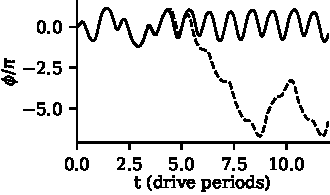
\includegraphics{chaos_pendulum}
  \caption{Two driven, damped pendulums released from angles that
    differ by one part in a thousand. For five drive cycles you cannot
    tell them apart; then one flips over the top and they never agree
    again. Week 14.}
  \label{fig:chaos}
\end{marginfigure}
\medskip
\marginnote{\textbf{Key dates}\\[2pt]
  \begin{tabular}{@{}ll@{}}
  Mon Oct 5   & Mountain Day holder\\
  Mon Oct 12  & No class (recess)\\
  Mon Oct 19  & Exam 1 (Ch.\ 2--4)\\
  Fri Nov 13  & Exam 2 (Ch.\ 5--7)\\
  Wed Nov 25  & No class\\
  Fri Nov 27  & No class\\
  Mon Dec 7   & Exam 3 (Ch.\ 8, 9, 11)\\
  Wed Dec 16  & HW13 due\\
  Dec 19--22  & Final exam period\\
  \end{tabular}\\[4pt]
  Mountain Day is announced the morning of; if it lands on a class
  day, that day's material shifts into the Oct 5 holder.}

\section{How the course works}\label{sec:machinery}

Everything in this course is worth points, and the course total is
exactly 1000 points. Within each category, each assignment is weighted
equally.

\medskip
{\small\noindent
  \begin{tabular}{@{}lrrrr@{}}
    \toprule
    \textbf{Category} & \textbf{Number} & \textbf{Drop} &
    \textbf{Each} & \textbf{Total}\\
    \midrule
    Participation \& pre-class check-ins (PCCIs) & 39 & 4 & 2 & 70\\
    Weekly homework & 13 & 1 & 25 & 300\\
    Exams (in class) & 3 & 0 & 190 & 570\\
    Final exam, required part (self scheduled) & 1 & 0 & 60 & 60\\
    \midrule
    \textbf{Course total} & & & & \textbf{1000}\\
    \bottomrule
  \end{tabular}
}
\medskip
\marginnote{\textbf{Grade scale} (not curved)\\[2pt]
  \begin{tabular}{@{}llll@{}}
  A  & 93+      & C+ & 77--79.9\\
  A- & 90--92.9 & C  & 73--76.9\\
  B+ & 87--89.9 & C- & 70--72.9\\
  B  & 83--86.9 & D+ & 67--69.9\\
  B- & 80--82.9 & D  & 63--66.9\\
     &          & D- & 60--62.9\\
     &          & E  & below 60\\
  \end{tabular}}

\subsection{Pre-class check-ins (PCCIs) and attendance}

\newthought{Most class days there will be a short PCCI due} at the start
of class, on paper: usually one Taylor problem, chosen so that working
it primes you for that day's material. \textbf{You will receive full
  credit for a good-faith effort that includes a clear description of
  anything you are stuck on.} An incorrect or incomplete answer
\emph{without} such an explanation won't receive full
credit.\sidenote{For example, if the question were to differentiate
  $f(g(x))$: ``I don't know'' earns nothing; the correct answer earns
  full credit; and so does ``I think it's $f'(g(x))$, except I know the
  chain rule says to do something different because it's $f(g(x))$ and
  not just $x$ -- I'm not clear on what, though.''} A PCCI should take
you less than 15 minutes; if one doesn't, please tell me. Turning in
the day's PCCI is also how attendance is recorded, and your four lowest
participation days are dropped, so occasional absences and off days
cost you nothing.

\newthought{This is a small class, and it runs on group work} at the
board. Your classmates are a resource for you and vice versa, and this
in-class work is one of the main benefits of a school like Smith. If
you have an accommodation, please come talk to me so that we can make
the class work for both of us, but \emph{in general}, I will expect you
to miss no more than four classes, and missing more than four may
adversely affect your grade.

\subsection{Weekly homework}

Physics is learned by doing problems, and upper-level mechanics
problems are long: expect a set of five or six Taylor problems each
week, most of them substantial. Homework is posted on Moodle and due
there \textbf{Wednesdays by 10:00~PM} as a single PDF of your written
work (photos of handwritten pages are fine; combine them into one
PDF). A few due dates move to sit before an exam or a break; the Moodle
calendar is authoritative.\sidenote{Most weeks one problem is
  \textbf{computational}, done in Python on \url{https://posit.smith.edu}.
  Include your code and its plots in the PDF. If you already know and
  prefer Mathematica, you may use it instead -- the physics is what's
  graded.}

You may (and should) work with others on the homework, but what you
submit must represent your own understanding, written up by you. Your
lowest homework score is dropped.

\newthought{Every problem ends with an assessment.} After the answer,
write two or three lines checking it: a limiting case ($m \to 0$, $t
\to \infty$, the angle going to zero), a units check, or a comparison
with a result you already trust. Some problems on the sets say
``include an assessment'' or ``this is your assessment''; the habit is
expected on all of them, and it is worth points in the rubric below.

\newthought{Homework is graded on correctness}, problem by problem, on
a simple scale:\sidenote{The rubric and the reflection option are Will
  Raven's, kept because they work: the students who wrote reflections
  were the ones whose exam scores moved.}
\begin{itemize}\small
  \item[$+$] 100\%: complete and correct, including units and the
    assessment.
  \item[$\checkmark$] 95\%: one small problem.
  \item[$-$] 50\%: several small problems, or one big one.
    \emph{Resubmitting a completely correct solution together with a
    few sentences of reflection raises this to 85\%.}
  \item[$\times$] 25\%: substantial confusion. \emph{A correct
    resubmission with an in-depth reflection raises this to 75\%.}
  \item[$0$] skipped.
\end{itemize}
A reflection says why the original attempt went wrong, what you were
thinking at the time, and -- most importantly -- what you now
understand that corrects it. Reflections and resubmissions are due
within ten days of getting the homework back, on separate pages
attached to the next set. A reflection without real engagement earns
less.

\subsection{Exams}

Three exams, in class, taking the full period, on the dates in the
margin above. Each exam has \textbf{three problems, one per chapter
  covered}; a student with command of the material should finish each
in about 25 minutes. Exams are closed-book; you may bring \textbf{one
  8.5$\times$11 sheet of handwritten notes, both sides}.\sidenote{You
  may use a basic calculator; no phones, laptops, or other
  internet-connected devices. Students with documented accommodations
  will, of course, have those accommodations met.} Exam problems are
closely aligned with the in-class problems and the homework, and each
exam covers only the chapters listed -- never the week the exam is
given.

\subsection{Final exam, with redemption problems}

The final, during the December 19--22 self-scheduled exam period, has
two parts:
\begin{enumerate}
  \item \textbf{Required} (60 points): one problem on Chapter 12
    (chaos), the only chapter not covered by an in-class exam.
  \item \textbf{Optional grade-replacement problems}: nine more
    problems, one for each chapter that appeared on the three exams
    (Chapters 2--9 and 11). Attempt any of them. For each one you
    solve, the new score \emph{replaces} your score on the
    corresponding exam problem if and only if it is higher. There is
    no penalty for an attempt; this can only improve your grade.
\end{enumerate}
Do the required problem first; then do as many redemption problems as
you want and have time for. I keep per-problem exam scores all
semester precisely so this works.

\subsection{Partial credit, and how to get it}

Several of the problems in this class are quite challenging. For the
harder problems, my goal is to have you make the strongest possible
effort toward \textbf{understanding} the solution. Thus, if you cannot
fully solve a problem, say whatever you can about the way in which a
solution would proceed from where you stop; say whatever you can about
the qualitative behavior of a solution; say whatever you can about the
physical meaning of the solution. And always, always: \textbf{check
  your units}, \textbf{check the limiting cases}, and \textbf{plug your
  solution back into the equation of motion}.\sidenote{You are never
  done solving an equation of motion until you have verified that your
  solution works.}

\subsection{Late policy}

It is extremely hard to catch up on late work (usually things are late
because you are busy, and people don't tend to get less busy!). That
is why every category has built-in drops: four participation days, one
full homework set. My strong suggestion, when life happens, is to use
the drops and prioritize getting your schedule back under control.

Beyond the drops: all students start the term with \textbf{3 free late
passes}. You can spend a late pass to extend a homework set to the
following class period with no penalty. Late passes are not automatic
-- email me before the deadline to say you're using one, and once
declared it is spent whether or not you turn the work in by the
extended date.\sidenote{Late passes cannot be applied to PCCIs (their
whole value is priming you for that day's class -- the drops cover
them), to exams, or to the final. After your free passes are spent,
further extensions cost 10\%, then 20\%, and so on, of that
assignment's points.}

\section{Python (and Mathematica)}\label{sec:python}

Computation is part of doing mechanics: the equations of motion for
quadratic drag, the driven pendulum, and the double pendulum have no
closed-form solutions, and numerical solutions are how physicists
actually see those systems. We will use Python (NumPy, SciPy,
Matplotlib) in Jupyter notebooks on \url{https://posit.smith.edu},
the same setup as PHY 210. I'll post starter notebooks for the
computational homework problems and for the in-class simulations.
Two expectations, borrowed from Will Raven's Mathematica policy for
this course:
\begin{enumerate}
  \item \textbf{Simplify first.} Anything that can be done with
    physics -- an integral that vanishes by symmetry, a limit you can
    read off -- gets done on paper first. The computer confirms; it
    does not replace your understanding.
  \item \textbf{Explore and assess.} Use the computer to push past the
    algebra: vary a parameter, plot the thing, check a limiting case
    numerically. Say in your write-up what you predicted \emph{before}
    running it and what you concluded \emph{after}.
\end{enumerate}
Previous offerings used Mathematica, and Smith has a license; if you
already know it and prefer it, you may use it for any computational
problem.

\section{A short statement on inclusion and equity}\label{sec:inclusion}

I can hardly overstate how much inclusion, equity and diversity
considerations have shaped my entire thinking around teaching and
practicing physics. It affects everything from the way that physics is
framed historically to the way that it is typically taught in your
classrooms. My main goal is to create an environment that tells all of
us that we can do physics; that invites people into physics who have
never been invited, or who have been explicitly excluded.

Physics cannot be divorced from the world in which we study it. I
expect that we will recognize that in this class, and I expect that we
will create an inclusive and welcoming environment. More specifically,
I expect that we will strive \textit{not} to create an environment that
excludes people. This is hard work. We will get things wrong. You will
get things wrong. \textit{I} will get things wrong. Especially when I
get things wrong, I encourage you to tell me, using any of the channels
under \emph{Sensitive issues} below.

\section{Use of artificial intelligence}\label{sec:ai}

Before we get to a policy, two things:

\begin{itemize}
  \item AI models make subtle errors, hallucinate, and hand you
    technically-correct solutions that teach you nothing; your job here
    is to verify, question, and ultimately understand the physics.
  \item Your PCCIs are graded on the basis of ``good-faith effort'',
    \textit{not} correctness -- the only thing I'm grading is a record
    of \emph{your} thinking, explicitly including credit for starting
    and then saying where you got stuck. Having AI polish that doesn't
    help your grade at all, and cheats you of learning. And the
    homework reflections only work if they are honestly yours.
\end{itemize}

So, the policy: AI is a powerful tool, and it offers real potential to
enhance your learning in this course. Used improperly, it can genuinely
hinder your development as a physicist. You are welcome to use AI in
this class, provided you always adhere to the Academic Integrity
Statement: \textbf{using AI to solve homework, PCCI, or exam problems
  is a violation of the Academic Integrity policy and will be treated
  as such}, and any AI use in work you submit must be cited, like any
other source.\sidenote{Adapted, with thanks, from Will Raven, whose
  ``AI prompts for students'' handout (on Moodle) is a good guide to
  using it \emph{well}: asking it to quiz you, to critique a
  reflection draft, or to pose ``what if'' variations of a problem you
  have already solved.}

We're happy to use AI where it actually helps in this class, but we
have to be careful not to use it before then. So, feel free to use AI
to dig further in, to get alternate explanations, to check rote algebra
after you've done it, to debug code by having it explain its diagnostic
process rather than hand you the fix, to explore new topics, etc. But
keep it in check to make sure you're in charge of your own learning.
Early in the semester, we will spend part of a class deciding
\emph{together} how AI should and shouldn't fit into homework in this
course -- computational work especially -- and we'll post what we
decide on Moodle next to this policy.

\section{Policies and logistics}\label{sec:policies}

\newthought{Communication.} My preferred mode of communication is
email. I will check my email multiple times per day during the work
week. If you have sent me an email and have not heard back from me
within 24 hours (excluding weekends), you should email me again or
drop by my office to ask your question in person. I cannot guarantee
that I will regularly check my email on evenings or on
weekends.\sidenote{I expect that you will check your Smith email at
least once per day: 24 hours after I email the class, I expect
everyone has read it. Emailed assignments, due dates, and policy
changes carry the same weight as this syllabus, and the same goes for
Moodle.}

\newthought{Workload.} This course should take about 12 hours of your
time per week: about 4 in class, and about 8 outside it on reading,
PCCIs, homework problems, and review. \textbf{If you find yourself
spending significantly more (or less) than this, please let me know
ASAP! That's an instructor-error that I can easily fix.}

\newthought{Sensitive issues.} What if you have something you want to
talk about, but don't feel comfortable doing so in a public (or
non-anonymous) space? This often comes up with issues of racism,
sexism, and other kinds of discrimination. It can come up with issues
that relate to my behavior, the behavior of your classmates, or the
world in general. Please feel \textit{encouraged} to use either the
anonymous feedback form linked on Moodle, or to leave a written note
under my door.\sidenote{If you want to write a note, you may want to
type it up and print it out so that your handwriting is further
anonymized.} Of course, if you feel comfortable and safe doing so, you
are also encouraged to talk publicly or non-anonymously about these
things! If you are not comfortable with any of these options, the
Resources section below lists offices that can help, including
confidential ones.

\newthought{Recording.} My plan is to record from my iPad to both PDF
and videos, posted to Moodle. We'll see how technology
works.\sidenote{I do this because several students have used it as a
post-class resource in the past. Sometimes a derivation is worth
reviewing, sometimes you were having a spacey day, etc. But it's worth
knowing that student experience shows that it's a very poor substitute
for attendance, and just watching the recordings won't count towards
your 70 attendance/participation points.} Sometimes the mic picks up
conversations in the room. If that's a problem, I can look into muting
it. Let me know.

\newthought{Academic Integrity.} Real learning happens when students
conduct themselves with academic integrity, and our goal here is to
provide you with the opportunity for (and expectation of) that
learning. Read the
\href{https://www.smith.edu/your-campus/offices-services/office-student-affairs/student-handbook/academic-honor-code-0}{Academic
  Integrity Statement}. That statement is a gift to the community,
giving you all sorts of privileges (self-scheduled finals, the
expectation that I treat you like academic adults, etc.). And it comes
with responsibilities.\sidenote{In this class specifically: you are
  encouraged to work together on the homework and to study together
  for exams, but PCCIs should be attempted individually first,
  everything you turn in must be your own work, and exams and the
  final must be done individually.}

\newthought{Academic accommodations.} If you need classroom
accommodations, please contact the
\href{mailto:ARC@smith.edu}{Accessibility Resource Center} and file
things through the
\href{https://smith-accommodate.symplicity.com/}{Accommodate system}. I
promise to be flexible in meeting any documented need for
accommodations in a way that works well for you. If you would like
some accommodation but do not have an ARC reference, let me know and we
can discuss your concerns: regardless, I want to provide you the
support you need to succeed in this course, though I will do so in a
way that does not diminish the accommodations of others. Remember to
contact me well in advance of when you need the accommodations in
place, so that we can prepare.

\newthought{Course feedback.} There will be an anonymous mid-semester
feedback form on Moodle around fall break, and during the last week of
classes approximately 15 minutes at the beginning of one class will be
set aside for you to complete the official course feedback
questionnaire. Please don't wait until then if something isn't
working.

\section{Recommended books, and other resources}\label{sec:resources}

\newthought{Books.} Taylor is unusually readable; most weeks the
reading is the best preparation you can do. When you want a second
voice: Morin, \textit{Introduction to Classical Mechanics}, has the
best problem collection in the subject (with solutions) and a more
demanding style; Kleppner \& Kolenkow, \textit{An Introduction to
  Mechanics}, is the classic at a slightly lower level and is excellent
on rotating frames and angular momentum; Marion \& Thornton,
\textit{Classical Dynamics of Particles and Systems}, is the
traditional alternative to Taylor and covers the same ground in a
different order. \textit{The Feynman Lectures on Physics, Volume I}
(free at
\href{https://www.feynmanlectures.caltech.edu/}{feynmanlectures.caltech.edu})
is worth reading on the principle of least action (Ch.\ 19 of Volume
II, actually) once we reach Lagrangians. Later in your career: Goldstein,
\textit{Classical Mechanics}, the graduate standard.

\newthought{People and places.} There are many resources at Smith to
help you succeed in this course and in your college career:
\begin{itemize}
  \item Your instructor! I am here to help you. That's my job, so
        don't think it's bothering me to have you reach out with
        questions or concerns.
  \item \todonote{course tutor / physics help-room hours, once
        scheduled.}
  \item The
        \href{https://www.smith.edu/academics/integrative-learning/spinelli-center-quantitative-learning}{Spinelli
        Center} -- open hours, one-on-one appointments, and math review
        workshops.
  \item Writing help, learning-specialist services, and workshops on
        time management and managing stress, all from the
        \href{https://www.smith.edu/academics/jacobson-center}{Jacobson
        Center}.
  \item Crisis resources,
        \href{https://www.smith.edu/your-campus/health-wellness/counseling-services}{counseling},
        and
        \href{https://www.smith.edu/your-campus/health-wellness}{wellness
        services} at the Schacht Center.
  \item Resources for
        \href{https://www.smith.edu/your-campus/offices-services/equity-inclusion/gender-identity-expression}{gender
        identity and expression}, and the
        \href{https://www.smith.edu/your-campus/offices-services/equity-inclusion}{Office
        for Equity and Inclusion} in general.
  \item \href{https://www.smith.edu/discover-smith/governance/institutional-policies/title-ix-smith-college}{Where
        to report sexual misconduct and other
        discrimination}. Please note that your instructors are
        \href{https://www.smith.edu/discover-smith/governance/title-ix-smith-college/responsible-reporters}{Responsible
        Reporters}.
\end{itemize}

\end{document}
